\section{DyNetKAT}

\begin{frame}{DyNetKAT}
    \begin{itemize}
        \item An extension to NetKAT to support dynamic and stateful behaviours
        \item Allows modelling and reasoning
              about control-plane updates and their interaction with data-plane flows
        \item Adds constructs for synchronisations and multi-packet behaviour
    \end{itemize}
    Syntax:
    \begin{align*}
        N & :: = \mathrm{NetKAT}^{-dup}                                 \\
        D & :: = \bot ~|~ N;D ~|~ x?N;D ~|~ x!N;D ~|~ rcfg_{x,N};D  ~|~ \\
          & D\parallel D ~|~ D \oplus D ~|~ \delta_{\mc{L}}(D)
        ~|~ \pi_n(D) ~|~ D \lm D ~|~ D | D ~|~ X                        \\
          & X \triangleq D, n \in \mathbb{N},
        \mc{L} = \s{c ~|~ c ::= x?N ~|~ x!N}
    \end{align*}
\end{frame}

\begin{frame}{DyNetKAT: Stateful Firewall}
    \begin{figure}
        \centering
        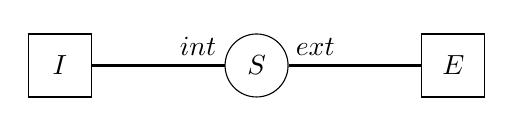
\begin{tikzpicture}[
                node distance={25mm},
                sw/.style = {draw, circle,minimum size=8mm},
                h/.style = {draw, rectangle,minimum size=8mm}
            ]
            \node[h] (i)  {$I$};
            \node[sw] (s) [right of=i]  {$S$};
            \node[h] (e)  [right of=s] {$E$};
            \draw [thick] (i)  -- node[above,pos=0.8]{$int$} (s);
            \draw [thick] (s) -- node[above,pos=0.2]{$ext$} (e);
        \end{tikzpicture}
    \end{figure}
    \begin{align*}
        Host  \triangleq   & secConReq!1;Host \oplus secConEnd!1;Host        \\
        Switch \triangleq  & (port = int) \cdot (port \la ext);Switch \oplus \\
                           & (port = ext)\cdot 0 ; Switch \oplus             \\
                           & secConReq?1;Switch'                             \\
        Switch' \triangleq & (port =int) \cdot (port \la ext);Switch' \oplus \\
                           & (port=ext)\cdot(port\la int);Switch' \oplus     \\
                           & secConEnd?1;Switch                              \\
        Init \triangleq    & Host \parallel Switch
    \end{align*}
\end{frame}
